\input{commun/presentations.tex}

\title[Séance 10 - Prépa vol]{Séance 10 \\ Préparation d'un vol}

\begin{document}
 \begin{frame}
 \titlepage
 \end{frame}
 
 \begin{frame}
 \tableofcontents
 \end{frame}
 
 \section{Préparation navigation}
	\begin{frame}{Vol Périgueux - Bordeaux Mérignac - itinéraire}
		\begin{itemize}
			\item Vol entre Périgueux LFBX et Bordeaux Mérignac LFBD
			\item L'avion vol à 120 kts
			\item Vent nul
			\item Déclinaison magnétique 5\degree est
			%\item Bonus : montée 500 ft/min à 90 kts
		\end{itemize}
		\begin{figure}[H]
			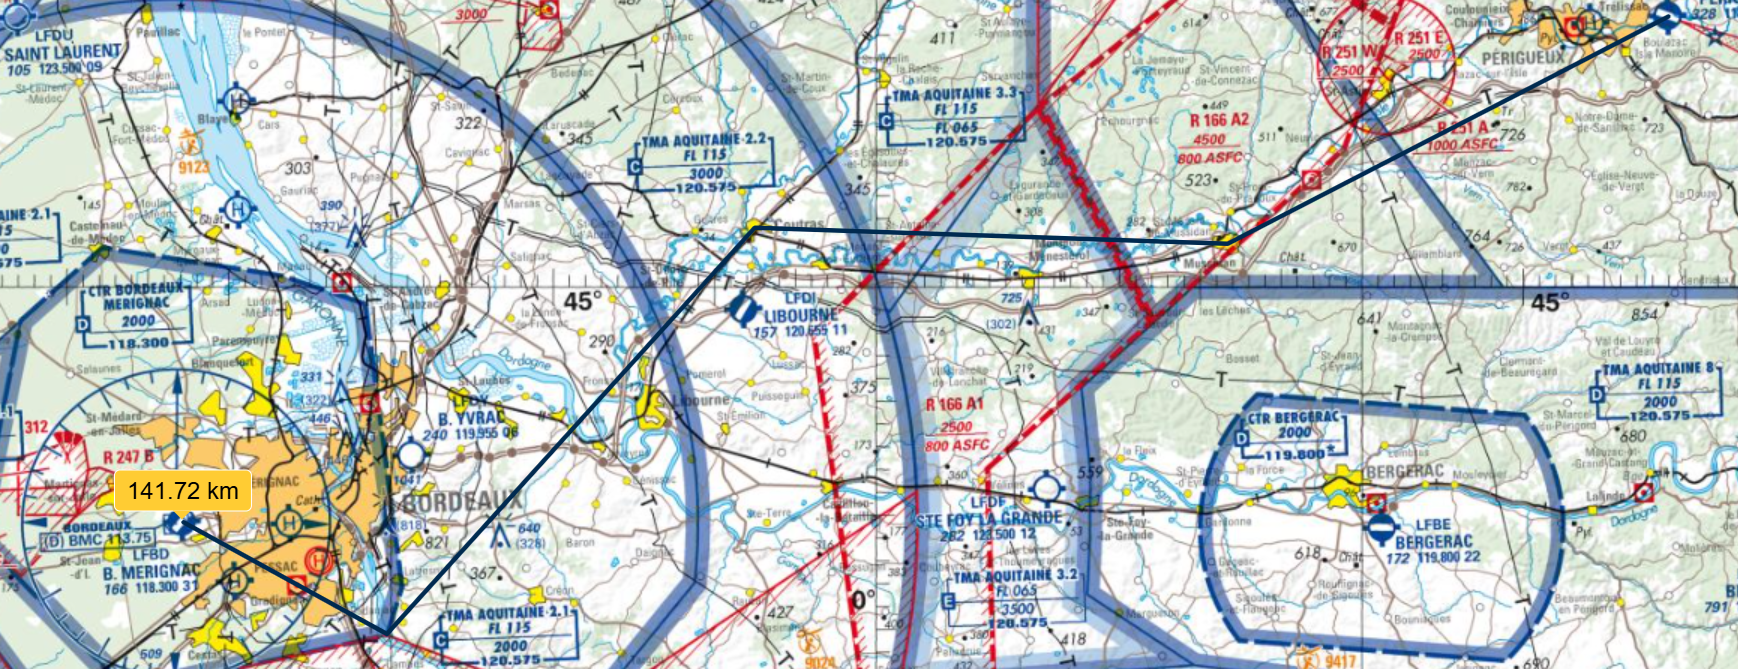
\includegraphics[width=0.7\linewidth]{imgPresentations/navigationLFBX-LFBD.png}
			\legende{Proposition d'itinéraire entre Périgueux et Bordeaux}{img:navigationLFBX-LFBD}
		\end{figure}		
	\end{frame} 	
	
	\begin{frame}{Vol Périgueux - Bordeaux Mérignac - itinéraire}
		\begin{figure}[H]
			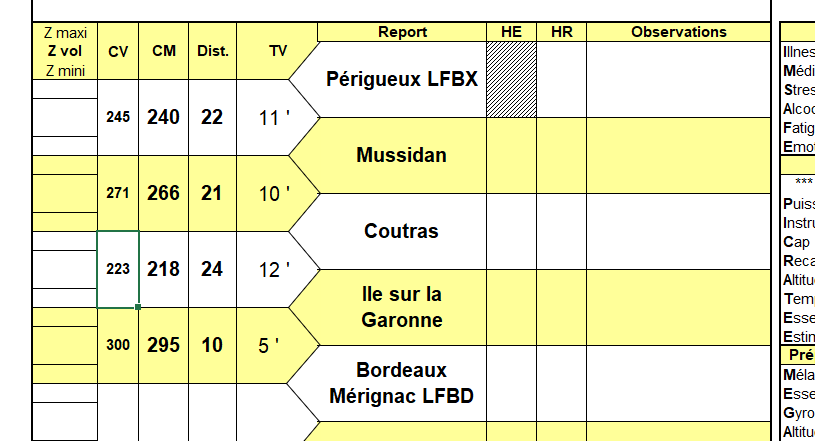
\includegraphics[width=0.9\linewidth]{imgPresentations/logNavLFBX-LFBD.png}
			\legende{Log de navigation entre Périgueux et Bordeaux}{img:logNavLFBX-LFBD}
		\end{figure}	
		
	\end{frame} 	
	
	\begin{frame}{Vol Périgueux - Bordeaux Mérignac - carburant}
		\begin{itemize}
			\item Consommation 40L/h
			\item Réserve finale de carburant 30 minutes	
		\end{itemize}	
	\end{frame} 	
	
	\begin{frame}{Vol Périgueux - Bordeaux Mérignac - carburant}
		\begin{figure}[H]
			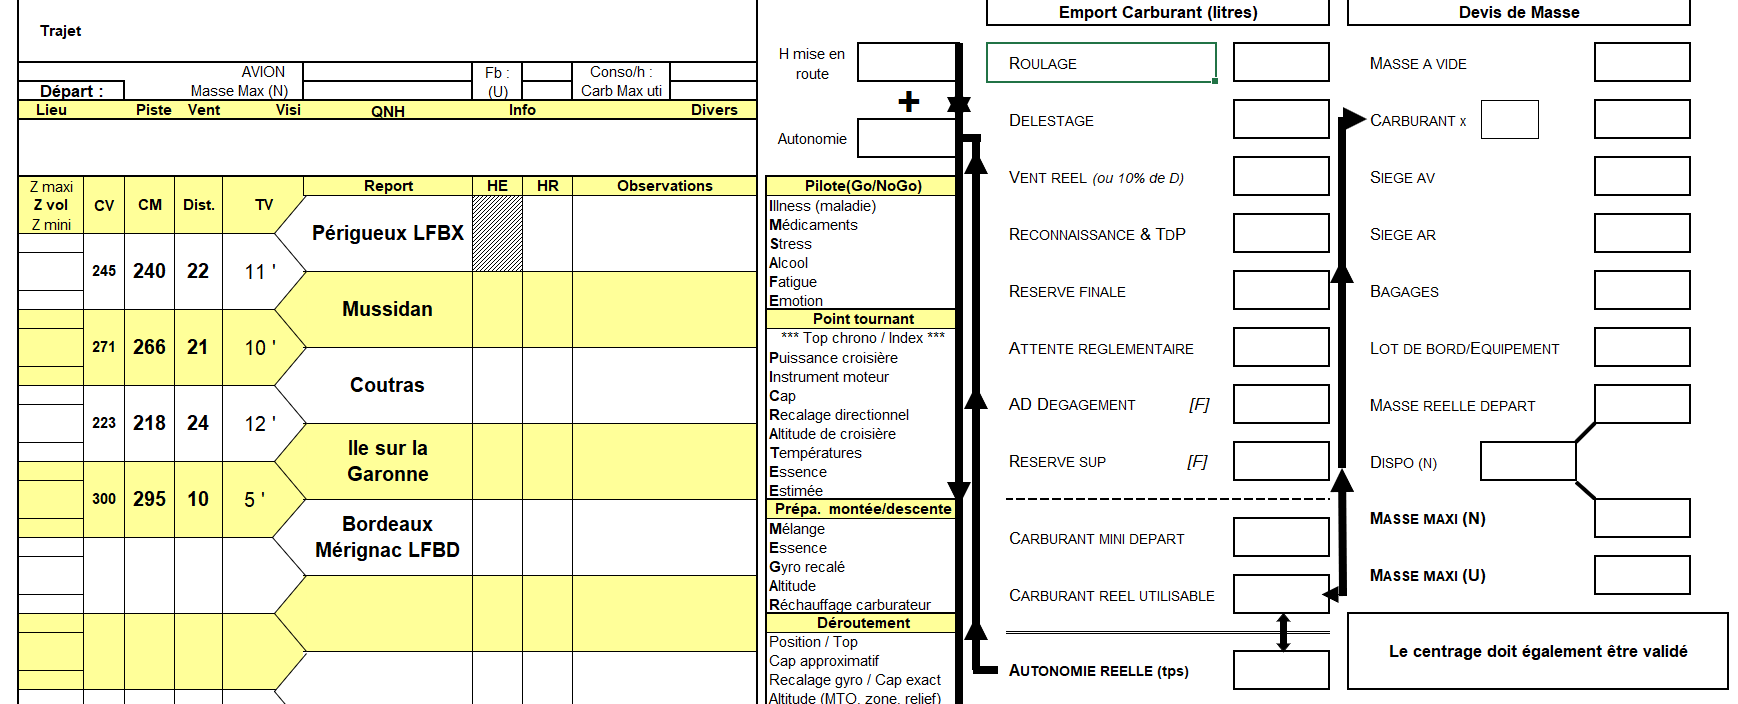
\includegraphics[width=1\linewidth]{imgPresentations/logNavCarbu.png}
			\legende{Log de navigation entre Périgueux et Bordeaux}{img:logNavCarbu}
		\end{figure}			
	\end{frame} 	
	
	\begin{frame}{Vol Périgueux - Bordeaux Mérignac - NOTAM}
		\begin{figure}[H]
			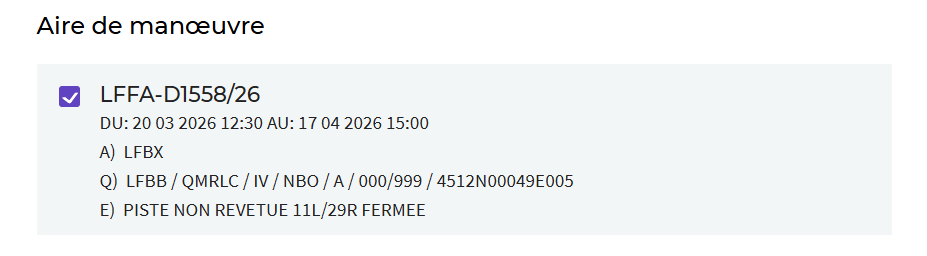
\includegraphics[width=0.5\linewidth]{imgPresentations/NotamLfbx.png}
			\legende{Exemple d'un NOTAM à Périgueux}{img:NotamLfbx}
		\end{figure}	
	\end{frame}
	
	\begin{frame}{Vol Périgueux - Bordeaux Mérignac - Météo}
		\begin{itemize}
			\item TEMSI
			\item Carte des fronts
			\item Wintem
			\item METAR et TAF	
		\end{itemize}			
	\end{frame}
	
	\section{Vol}
	\begin{frame}{Vol}
		\begin{itemize}
			\item Visite Prévol \pause \faCheck
			\item Mise en route \pause  \faCheck
			\item Essais moteurs \pause \faCheck
			\item Roulage \& Décollage
		\end{itemize}
	\end{frame}
	
	\begin{frame}{Carte VAC Périgueux}
	\begin{columns}
		\begin{column}{0.5\textwidth}
			\begin{figure}[H]
				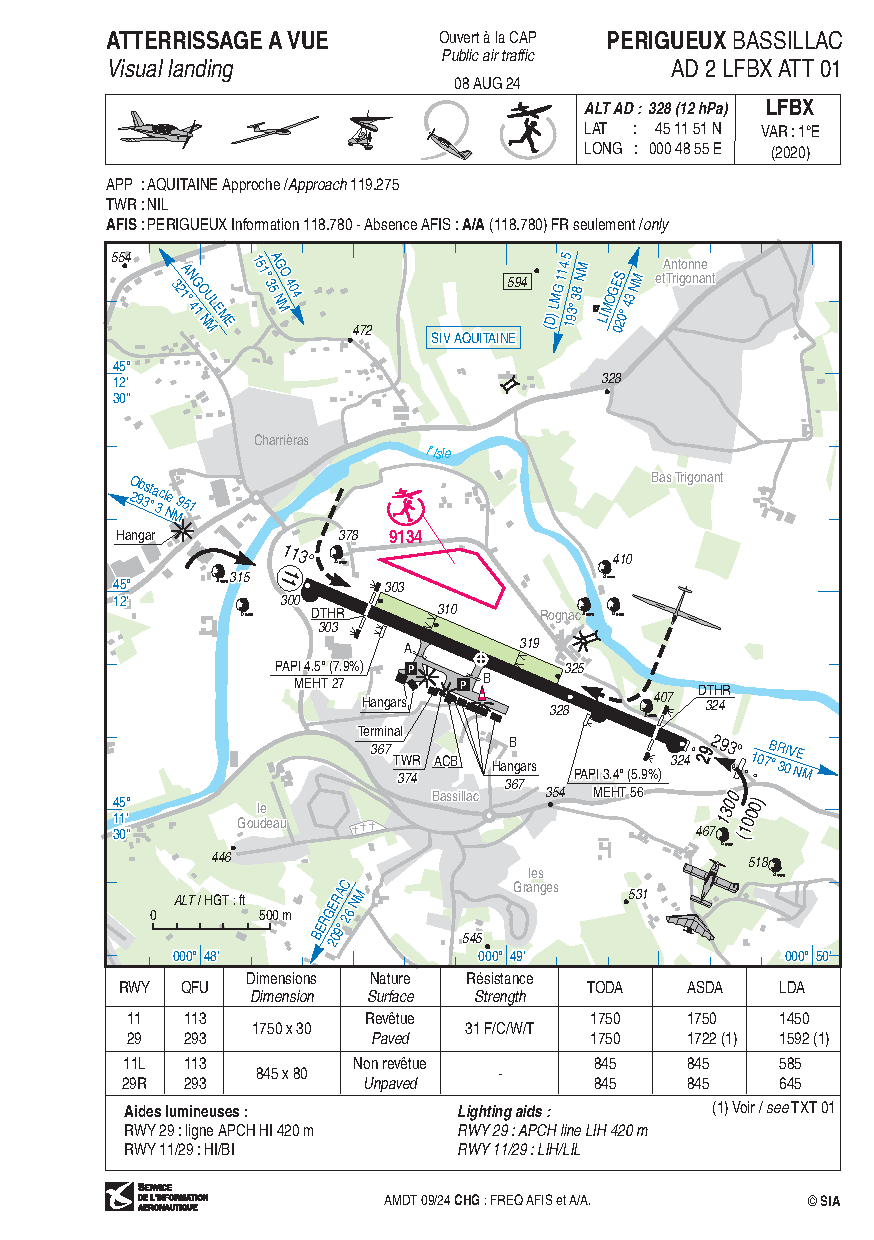
\includegraphics[width=0.7\linewidth,page=1]{imgPresentations/vacLfbx.pdf}
				\legende{VAC Périgeux, page 1}{img:vacLfbx}
			\end{figure}	
		\end{column}
		\begin{column}{0.5\textwidth}
			\begin{figure}[H]
				\includegraphics[width=0.7\linewidth,page=2]{imgPresentations/vacLfbx.pdf}
				\legende{VAC Périgeux, page 2}{img:vacLfbx}
			\end{figure}	
		\end{column}
	\end{columns}
	\end{frame}
	
	\begin{frame}{Vol}
		\begin{itemize}
			\item Visite Prévol \faCheck
			\item Mise en route \faCheck
			\item Essais moteurs \faCheck
			\item Roulage \& Décollage \pause \faCheck
			\item Navigation \pause \faCheck
			\item Procédure d'arrivée
		\end{itemize}
	\end{frame}
	
	\begin{frame}{Carte VAC Bordeaux Mérignac}
	\begin{columns}
		\begin{column}{0.33\textwidth}
			\begin{figure}[H]
				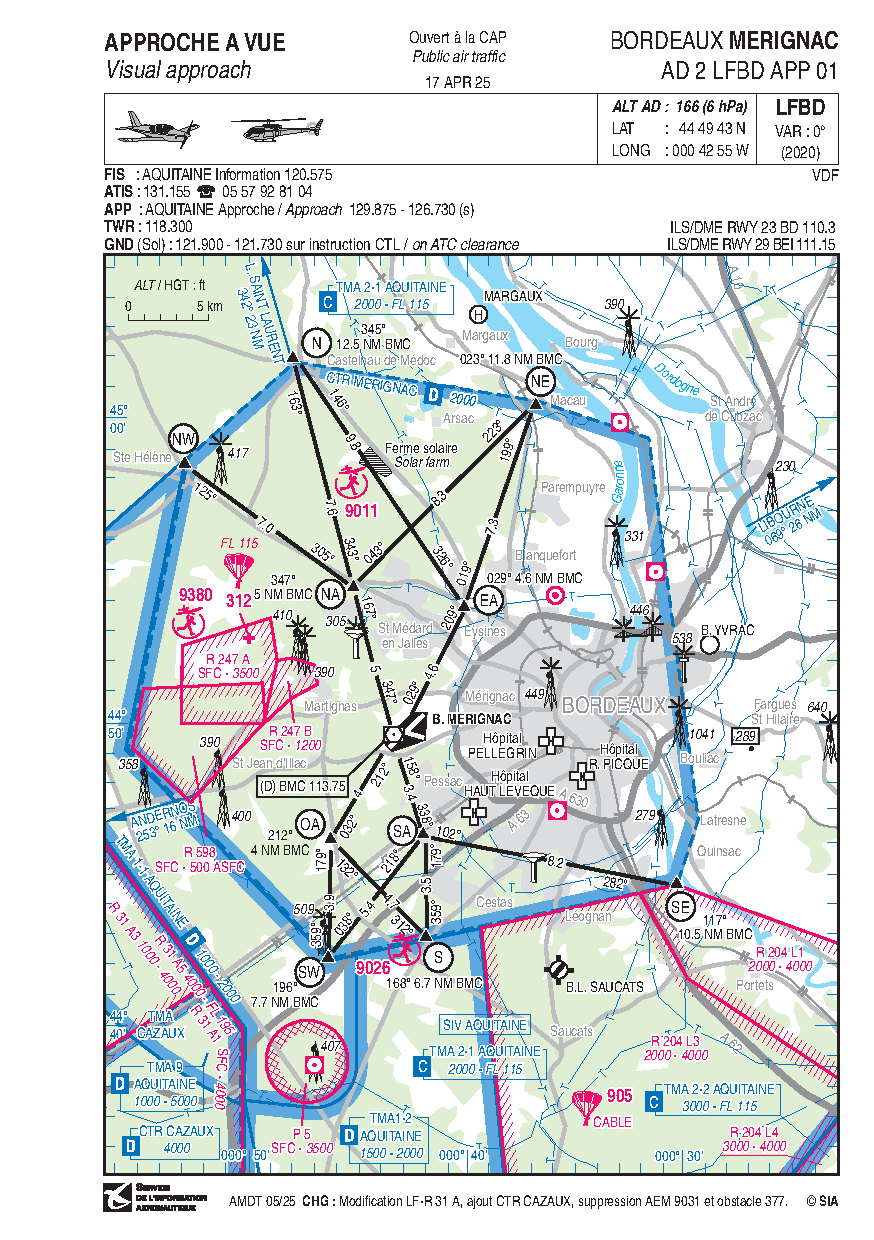
\includegraphics[width=1\linewidth,page=1]{imgPresentations/vacLfbd.pdf}
				\legende{VAC Mérignac, page 1}{img:vacLfbd}
			\end{figure}	
		\end{column}
		\begin{column}{0.33\textwidth}
			\begin{figure}[H]
				\includegraphics[width=1\linewidth,page=2]{imgPresentations/vacLfbd.pdf}
				\legende{VAC Mérignac, page 1}{img:vacLfbd}
			\end{figure}	
		\end{column}
		\begin{column}{0.33\textwidth}
			\begin{figure}[H]
				\includegraphics[width=1\linewidth,page=3]{imgPresentations/vacLfbd.pdf}
				\legende{VAC Mérignac, page 3}{img:vacLfbd}
			\end{figure}	
		\end{column}
	\end{columns}
	\end{frame}
	
	\begin{frame}{Vol}
		\begin{itemize}
			\item Visite Prévol \faCheck
			\item Mise en route \faCheck
			\item Essais moteurs \faCheck
			\item Roulage \& Décollage \faCheck
			\item Navigation \faCheck
			\item Procédure d'arrivée \pause \faCheck
			\item Approche et atterrissage \pause \faCheck
		\end{itemize}
	\end{frame}
	
\appendix 
%\section{QCM}
%\qmcBia{Navigation, réglementation, sécurité des vols}
%{1}{Pour la sécurité des vols, la qualité qu'il faut avoir en priorité est :}
%{une bonne connaissance de soi, de ses limites et de sa machine}
%{une grande habileté de pilotage}
%{un grand nombre d'heures de pilotage}
%{une bonne connaissance de la réglementation} 
%{}



 
\input{commun/beamerSlidesBiblio.tex} 
 
\end{document}
